\documentclass[acmtocl]{acmtrans2m}
%&t&{\tt #}&
%&v&\verb|#|&

% fancybox prevents the TOC from printing
%\usepackage{fancyhdr, fancybox, tabularx, verbatim, epsfig}
\usepackage{fancyhdr, tabularx, verbatim, epsfig}
\usepackage{amssymb,psboxit}
\usepackage{rotating}

\acmVolume{0}
\acmNumber{0}
\acmYear{00}
\acmMonth{00}

\newtheorem{interface}{Interface}[section]
\newtheorem{remark}{Remark}

\newcommand{\BibTeX}{{\rm B\kern-.05em{\sc i\kern-.025em b}\kern-.08em
    T\kern-.1667em\lower.7ex\hbox{E}\kern-.125emX}}

\markboth{}{Interfaces to Sparse Direct Solvers}

\title{On the Design of Interfaces to Sparse Direct Solvers}

\author{}

\begin{abstract}
We report on the design of general, flexible, consistent and efficient
interfaces to direct solver algorithms for the solution
of distributed and sparse systems of linear equations. We suppose that such algorithms are available
in form of software libraries, and we introduce a framework to facilitate the
usage of these libraries. This framework is composed by two key components:
an abstract matrix interface to access the
linear system matrix elements, and an abstract solver interface that controls
the solution of the linear system. 

We describe a concrete implementation of
the proposed framework, which allows a high-level view and usage of most of
the currently available libraries that implements direct solution methods for
linear systems. We comment on the advantages and limitation of the framework,
and we report several numerical results to show that the overhead required by
the interface is negligible.

\end{abstract}


\category{D.1.3}{Programming Techniques}{Parallel Programming}
\category{D.2.2}{Software Engineering}{Design Tools and Techniques--{\sl
 Object-oriented design methods}}
\category{D.2.13}{Software Engineering}{Reusable Software--{\sl Reusable
  libraries}}
\category{G.1.3}{Numerical Analysis}{Numerical Linear Algebra--{\sl 
  Sparse, structured, and very large systems (direct and iterative methods)}}
\category{G.4}{Mathematical Software}{Algorithm design and analysis}

%\terms{Documentation, Languages}

\keywords{Multilevel preconditioners, object-oriented}
\begin{document}


\setcounter{page}{1}

\begin{bottomstuff}
Author's address: 
\end{bottomstuff}

\maketitle

% --------------------------------------------------------------------------- %
\section{Managing Direct Solver Libraries}
\label{sec:introduction}
% --------------------------------------------------------------------------- %

In this paper we report on the design of general, flexible, consistent and
efficient interfaces to serial and parallel direct solver algorithms for
sparse linear systems of type
\begin{equation}
  \label{eq:linear_system}
  A X = B,
\end{equation}
where $A \in \mathbb{R}^{n \times n}$ is a real, square matrix, 
  and $X \in \mathbb{R}^{n}$ and $B \in \mathbb{R}^{n}$  are the solution and
right-hand side vectors, respectively. 

Generally speaking,
a direct solver algorithm for (\ref{eq:linear_system}) is any 
technique that defines three matrices, $L$, $D$ and $U$, so that
$A = L \, D \, U$, and the linear systems with matrices $L$, $D$ and $U$ are
easy to solve. Generally, $L$ is a lower triangular matrix, $U$ is an
upper triangular matrix, and $D$ is a diagonal matrix 
(or possibly the identity matrix), and the algorithms adopted for their
computation is some variant of the Gaussian elimination
process~\cite{xxx}. 

Developing direct solvers for problem (\ref{eq:linear_system}) is a
challenging task that has been a subject of research for the
past four decades. Serial dense linear systems can be solved with the
widely-available suite of solvers of the LAPACK
library~\cite{lapack-guide}, while distributed dense linear system can be
tackled using the ScaLAPACK library~\cite{scalapack-guide}.

For sparse matrices the situation is significantly different.
In general, the implementation of direct algorithms
requires much more expertise, longer time, and more resources than other
numerical analysis algorithms.  In this article we do not discuss
factorization algorithms, and we refer
to~\cite{amestoy01analysis,gupta01recent} and the references therein for more
details.  
Even if significant breakthroughs have been made during the last years,
it is still very challenging to implement direct solver algorithms
on a single processor, yet alone on multiprocessor machines. 
Unfortunately, the simple question of what is the best direct solver library
has no definite answer.

In this paper, we consider the point of view of application developers that
are interested in the {\sl usage} of already-available libraries.
The usage of a direct solution library has usually been conducted by writing a
custom-made adaptor between the library and the final application.
Basically, one
has to form the linear system matrix using the storage format required by the
library, then call the correct sequence of instructions to factorize the matrix
and solve the linear system.  The approach is sub-optimal because it leads to:
\begin{itemize}

\item 
{\sl Replicated Code.}
Direct solution methods are required by several numerical algorithms. An
incomplete list would include
implicit time-marching schemes, 
Newton-like methods, multilevel and domain decomposition preconditioners.
Writing an adaptor from each of these applications to a given library  
(or to a  set of libraries) leads to replicated code, which is difficult
to test, debug, and maintain.

\item 
{\sl Difficult Testing.}
It is often difficult to choose the best direct solver library among the
several existing projects.  In some cases, a theoretical analysis of
the problem at hand can suggest the right algorithm; alternatively, one can
consider numerical comparison available in the literature
on test matrices. Often, however, the best
choice is to test a given solver on the application, architecture, and data
set of interest, and this can be done only if an adaptor  to a library
implementing the given method is already available.

\item 
{\sl Maintenance Problems.}
Including the adaptors within the application code requires the application
developers to take care of several details, like matrix format, memory
management, calling sequence, header files, and so on, that can vary 
from one version to the next. 

\item {\sl Partial Coverage}. Writing an adaptor means that only a library or
a set of library are targeted, and all other projects are discarded. 
\end{itemize}

The approach advocated in this paper is instead to introduce an interface
between the applications and the direct solver libraries, so that each
library can be encapsulated within the interface. Each interface (or adaptor)
  will take care of dealing with the direct solver library, in a manner that
  is transparent to the application developer.  
The proposed set of interfaces
can be used to access a wide variety of
well-know libraries of direct solution methods. The interface is clean and
consistent for all libraries, and automatically manage matrix formats, data
layout, calling sequences, and all the other ``details'' required by the
supported libraries. Our final goal is the
definition of an easy-to-use and efficient framework between them and the
applications. 

\medskip

This document presents how these interfaces can be
defined.  Our starting point is the rich set of libraries made available by
several researchers. These projects are briefly reviewed in
Section~\ref{sec:review}.  The interfaces are presented in
Section~\ref{sec:design}. A concrete implementation of these interfaces is
presented in Section~\ref{sec:concrete}.  Note that we explicitly avoided to
report any numerical comparison using these libraries, since this task
is extremely challenging and application dependent. Finally,
  conclusions are drawn in Section~\ref{sec:conclusions}. 

%-----------------------------------------------------------------------------
\section{Brief Overview of Direct Solution Methods}
\label{sec:theory}
%-----------------------------------------------------------------------------

{\bf Ken, this section is still needs references}

Direct solvers use Gaussian elimination (\ref{eq:ldu}) followed by a
forward solve (\ref{eq:forward}) and a backsolve (\ref{eq:backward})
to solve a system of linear equations (\ref{eq:orig_eq}):

\begin{eqnarray}
  \label{eq:orig_eq}
  A X = B \\ 
  \label{eq:ldu}
  PAQ = LDU \\
  \label{eq:forward}
  LX_1 = PB \\
  \label{eq:backward}
  UQ^{-1}X = D^{-1}X_1  
\end{eqnarray}

Where: $P$ and $Q$ are permutations.  $L$ and $U$ are lower and upper triangular, respectively.  And, $D$ is diagonal (often the identity matrix).  

If $A$ is sparse, $L$ and $U$
are typically sparse, though they may have some fill-in, i.e. non-zero entries which are zero in
$PAQ$.  

In a typical solver for an unsymmetric matrix, the column permuation,
$Q$ is chosen to minimze fill-in, while $P$, the row permutation, is
chosen to maintain numerical stability.  

Most direct solvers perform Gaussian elimination ($LU$ decompostion) in
two phases.  Symbolic factorization analyzes the matrix (typically
looking only at the structure or non-zero pattern of the matrix).
Numeric factorization uses the information from the symbolic
factorization phase, usually including a fill reducing column permutation, 
to improve performance.  

The performance of a sparse direct solver depends on the underlying
matrix, computer, application, algorithms, and libraries as well as
the code and how it is compiled.  Although a solver designed for an
unsymmetric matrix will work on symmetric matrices, solvers designed
for symmetric matrices will typically be faster on symmetric matrices.
Codes designed for shared memory computers will not run on distributed
memory computers.  Codes designed for distributed memory computers can
work on shared memory computers, but cannot take full advantage of the
shared memory architecture.  Many applications require repeated solves
with little or no difference in the matrix between solves.  Some
algortihms are able to take advantage of the similarity in matrices
between solves.

The different charasteristics of the matrices which users wish to
solve impact sparse direct solvers.  Some matrices are symmetric in both
structure and data $A_{i,j} = A_{j,i}$ for all $i$ and $j$.  Some of
the symmetric matrices are positive definite, SPD, and require no
pivoting.  The most efficient algorithms for symmetric and SPD
matrices will not work on other matrices.  Some are symmetric in
structure, $A_{i,j} == 0$ iff $A_{j,i} == 0$, or nearly so.
Algorithms that maintain symmetry typically outperform others on
matrices with symmetric or nearly symmetric structure.  Some have many
columns and/or rows that are structurally identical, or nearly so.
Aggregating nearly identical rows and columns into blocks allows more
efficient BLAS3 routines to be used.  Some can be factored with little
fill-in, others require significant fill-in.  Matrices that can be
factored with litte fill-in and have few identical or nearly identical
rows and columns are best handled by a low overhead code that does not
use the BLAS.  Some matrices are banded or nearly so, allowing the use
of a banded solver.  Matrices that have a non-trivial reduction to
block triangular form can be solved more quickly, often dramatically,
by a solver that includes reduction to block triangular form.  No sparse direct solver is best for all types of matrices.  

Some sparse direct solvers are designed for single processor
computers, some are designed for shared memory computers and others
are designed for distributed memory computers.  Solvers designed for
single processor computers can, if they use the BLAS for much of their
computation will achieve some speedup on shared memory computers.
Likewise, solvers designed for distributed memory computers can work
on shared memory computers using an MPI interface.  However, only
codes designed for shared memory computers can take advantage of the
shared memory architecture.  But, codes designed for shared memory
computers will not work on distributed memory computers.  No single
code will provide optimal performance across all architectures.

Some solvers handle certain application requirements better than
others.  Most aplications perform a series of solves, possibly
involving similar or even identical matrices.  If the matrix does not
change between two consequetive solves, the symbolic and numeric
factorization phases need not be performed for each solve.  If the
structure of the matrix does not change between consequetive solves,
but the values do, the numeric factorization must be performed for
each solve, though the symbolic factorization phase need not be.  If
the matrix values change, but the change is modest, the pivot order
may not need to change.  Therefore, some applications care most about
the execution time of the solve phase, while others are most sensitive
to the execution time of the factorization (numeric and/or symbolic).
Some applications require more accuracy than others.


\subsection{Solver strategies}

Sparse direct solvers are complex codes which use a number of
strategies to reduce memory and time costs.  Pivoting for numerical
stability makes it impossible to know in advance how the algorithm
will proceed and requires a flexible data structure.  This is
particularly difficult for distributed memory codes.  

Solvers use different strategies to reduce fill-in.  Many ordering
methods exist to reduce fill-in and most sparse direct solvers support
more than one.  Some solvers will even choose an ordering method for
you.  There are multiple variations on minimum degree orderings: AMD,
COLAMD, MMD and variants within these.  Graph partitioning algorithms
result in bi-section or multi-section based orderings.  Solvers
designed for symmetric and nearly symmetric matrices typically use
symmetric permutations to maintain symmetry.  No single ordering
method s best for all matrices, nor has a heuristic been found that
consistently chooses the best ordering.

Since pivoting adds complexity which significantly increase execution
time, many solvers offer options to reduce the cost of pivoting.  Some
equilibrate the rows and columns of the matrix to improve diagonal
dominance.  Many codes will consider the effect on execution time when
choosing a pivot, accepting some loss of numerical stability.
Typically this just means accepting the diagonal pivot if it is within
some threshold of the best available, but some codes will take the
predicted effect on execution into consideration when choosing an off
diagonal pivot.

Some codes combine similar rows and columns into blocks to improve
locality and allow high performing BLAS to be called.  Some combine
only rows and columns that are identical, others will accept minor
differences in the rows and columns that they treat as blocks.  Such
blocking can reduce the cost of symbolic factorization as well.

The three common methods for exploiting parallelism are the
multi-frontal method, coalescing  similar 
columns into blocks and calling a parallel dense solver 
to factor the final block of the matrix.

Some solvers allow incomplete factorizations which ignore small
elements in the original matrix and/or the $L$ and $U$ factors.
This feature is used primarily by users seeking a
preconditioner for an iterative method.

Some solvers use iterative refinement to improve accuracy.  Iterative
refinement is used most often with codes that do not perform full partial pivoting.  

Given the differences in matrix, computer, application, algorithms,
and libraries, it is unlikely that a single sparse direct solver will 
outperform all others across all usages.  





%-----------------------------------------------------------------------------
\section{Review of Considered Direct Solver Libraries}
\label{sec:review}
%-----------------------------------------------------------------------------

{\bf Ken, also this section is very incomplete...}
\bigskip

This Section gives an overview of some of the direct solver libraries
we have considered to develop our set of interfaces.
Our interest in mainly in sparse matrices; however, we have also considered
two well-known libraries for dense matrices. For processor communication, our
main interest is in MPI-based libraries.

There are several direcdt sparse solver packages freely available; other
software is commercial and it is not considered here. We have considered the
following libraries:

\begin{itemize}
\item
{\sl UMFPACK}. This is a general unsymmetric, multifronal, system-solver
package~\cite{umfpack-home-page}. It is written in C, and it is a sequential
package.
\item
{\sl PARDISO}. This sequential package is written in
C~\cite{oskl:04-etna,sg:04-fgcs}.
\item
{\sl TAUCS}. This sequential C package is targeted to symmetric matrices;
see~\cite{irony04parallel,rotkin04design,rozin04locality}.
\item 
{\sl SuperLU} and {\sl SuperLU\_DIST}. This solver~\cite{superlu-manual} is
available in single-processor, multithreaded version, and parallel version
using MPI. By use of supernodes and panel updates, which enable the use of
level-3 BLAS, it achieves a high performance. This package can handle fairly
general matrices.
\item
{\sl MUMPS}. This FORTRAN90, MPI package can handle symmetric and general
matrices.
\item
{\sl DSCPACK}. This C solver using MPI is targeted to symmetric matrices, and
uses the concept of domain separators to achieve parallelism.
\item
Other solvers are: {\sl SPOOLES}, {\sl WSMP}, {\sl Y12m}, {\sl PSPASES}.
\end{itemize}

We have here considered these libraries because of two reasons.
First, these codes use different algorithms that are
representative of a far wider range of codes. Second, these libraries are
among the best codes publicly available, and are widely used. 

By analyzing these projects, one can observe that:
\begin{itemize}
\item {\sl Different programming languages are used,}  even if C appears to be
  the language of choice of developers in this community.

\item {\sl Different communication paradigm are used.} 
 Most of the reviewed libraries are serial, some are based on the MPI
 paradigm, some other can take advantage of shared memory computers.

\item {\sl Different matrix formats are required.} Some libraries require the
so-called CSR format, other the so-called COO format. 

\item {\sl Different data layout.} Not all solvers can take advantage of
parallel environments. Those that do, often require different distribution of
data. 

\item {\sl Different Calling Sequence.} The exact calling sequence varies
widely from one library to the next.  Some libraries offer more than one way
to access the factorization and solution phases.

\item {\sl Different algorithms.} The underlying algorithms are radically
different...

\end{itemize}

%-----------------------------------------------------------------------------
\section{Project Design}
\label{sec:design}
%-----------------------------------------------------------------------------

We aim to construct a framework that allows a transpart and consistent usage
of most of the libraries presented in Section~\ref{sec:review}, and makes it easy
to extend the support to other (new) projects. We require the following capabilities:
\begin{itemize}

\item {\sl Simplicity of usage:} Solving linear system (\ref{eq:linear_system}) in a language
like MATLAB is very easy, just write \verb!X = A \ b!. It should not be much
more difficult in a production code.

\item {\sl Flexibility:} More than one algorithm must be available,
  to offer optimal algorithms for small and large matrices, serial and
  parallel.

\item {\sl Efficiency:} The solution of (\ref{eq:linear_system}) must be as
efficient as possible, using state-of-the-art algorithms. Besides, the
overhead due to the design must be minimal.
\end{itemize}

We will present our design as a set of C++ classes. We adopted C++ because it
supports object-oriented design, and it is relatively easy to interface
FORTRAN77, FORTRAN90 and C libraries with C++ code. C++ is nowadays a common
choice for developers  of scientific libraries and applications, and several
projects have adopted C++ as the language of
reference~\cite{heroux05trilinos}. As regards the model of parallel computing,
we consider parallel architectures with distributed memory, and we suppose
that a message passing interface (usually MPI~\cite{mpi-forum}) is adopted.
This approach is followed by the most important scientific libraries currently
available~\cite{heroux05trilinos,petsc-user-ref,falgout02hypre}; as a result, the presented
design can be easily interfaced with the aforementioned projects.

\bigskip

Our set of interfaces is based on the following classes: a {\tt Map}, which
defines the data layout of distributed objects among the available processes,
and {\tt Vector}, which standarizes objects like $X$ and $B$ in
(\ref{eq:linear_system}), a {\tt RowMatrix}, which is a data-independent
matrix interface, a {\tt Redistributor}, which encapsulates all the operations
required to redistribute {\tt Vector}'s between two different {\tt Map}'s, and
a {\tt Solver}, that connects the application code to the library of interest.
These classes are described in the following sections.

%-----------------------------------------------------------------------------
\subsection{The {\tt Map} Class}
%-----------------------------------------------------------------------------

The first object that we need to introduce is a {\tt Map}, which contains the
set of local indices, and a local-to-global mapping. The simplest map is a
linear map, which assigns contiguous subsets of nodes to the different
processors; however the implementation should be general enough to tackle more
general maps. A map object will implement the following interface.

\begin{interface}
\label{int:map}
The {\tt Map} class will contain the following methods:

\begin{itemize}
\item {\tt int GetNumMyElements()} returns the locally owned elements;
\item {\tt int GetNumGlobalElements()} returns the global number of elements;
\item {\tt int GetGID(int LID)} returns the global ID of local node {\tt ID}.
\end{itemize}
\end{interface}

%-----------------------------------------------------------------------------
\subsection{The {\tt Vector} Class}
%-----------------------------------------------------------------------------

As long as a map object is defined, one can create distributed vectors, that
are locally defined as arrays of {\tt double}'s. The simplest set of methods
of a vector is specified in Interface~\ref{int:vector}.

\begin{interface}
\label{int:vector}
The {\tt Vector} class will contain the following methods:

\begin{itemize}
\item {\tt double* GetValues()} returns a pointer to the local array of values;
\item {\tt Map\& GetMap()} returns a reference to the underlying Map object.
\end{itemize}
\end{interface}

For the sake of simplicity, this paper focuses on vectors and not on
multi-vectors (that is, a collection of vectors with the same {\tt Map}).
However, the presented design can be extended straightforwardly to tackle
multi-vectors.

%-----------------------------------------------------------------------------
\subsection{The {\tt RowMatrix} Class}
%-----------------------------------------------------------------------------

We can now define the most important interface of this paper: the {\tt
  RowMatrix} class. We decided not to impose any rigid matrix format.
In fact, although converting a matrix from
one given format to another is not a difficult operation, it is still a burden
that can slow down or prevent the usage of a package. Our object is to define
a unified interface so that the user does not have to worry about the internal
matrix format of a given package. As concerns the
data layout, we would like to have the be able to let users provide the linear
system as it is most convenient to their needs, then let the framework will
take care of data redistribution.  

Because of the way a Map is defined, the linear system matrix $A$ is
distributed
across the processor by assigning each row to a different processor.
We suppose that $A$ is available in local ordering.
Therefore, each local matrix can be decomposed as
\begin{equation}
A^{(loc)}_i + A^{(ext)}_i,
  \end{equation}
where $A^{(loc)}_i$ represents the square submatrix of elements whose row
and column correspond to locally hosted rows. The number of columns of
$A^{(ext)}_i$ containing at least one nonzero element defines the number of
the so-called {\sl ghost nodes}.

\smallskip

The abstract matrix interface is as
follows. Function names are reported
without the list of parameters to simplify the discussion.

\begin{interface}
\label{int:ami}
The abstract interface to the distributed square matrix $A$
will contain the following methods:
\begin{itemize}
\item \verb!int GetNumMyRows()! returns the number of locally hosted rows;
\item \verb!int GetNumGlobalRows()! returns the global number of rows;
\item \verb!int GetNumGhostNodes()! returns the number of ghost nodes;
\item \verb!void GetUpdateGhostNodes(Vector& X)! updates the values of ghost nodes
 in the input vector {\tt X};
\item {\tt void GetMyRow(int ID, int\& NumEntries, int* Indices, double*
                             Values)} copies the
columns and values of all nonzero elements in locally hosted row 
in the user's allocated arrays.
\item \verb!Map& GetRowMap()! returns a reference to the map;
\item \verb!Map& GetColMap()! returns a reference to the map for the columns
(which contains the ghost elements).
\end{itemize}
\end{interface}

%-----------------------------------------------------------------------------
\subsection{The {\tt Redistributor} Class}
%-----------------------------------------------------------------------------

Finally, we suppose that, given two maps, called SourceMap and TargetMap, a
{\tt Redistribute} object can be used to redistribute a {\tt Vector} based on
{\tt SourceMap} to a vector based on {\tt TargetMap}. This class encapsulates
all the complexity of data communication.

%-----------------------------------------------------------------------------
\subsection{The {\tt Solver} Class}
\label{sec:asi}
%-----------------------------------------------------------------------------

We can now describe the class that control the direct solver itself.
We recall that our main goal is the make the calling sequence required to
factorize and solve (\ref{eq:linear_system}) as clean and consistent as
possible.
To fulfill this design requirement, we split the solution
of linear system (\ref{eq:linear_system}) into the
following steps:
\begin{enumerate}
\item Definition of the sparsity pattern of the linear system matrix;
\item Computation of the symbolic factorization;
\item Definition of the values of the linear system matrix;
\item Computation of the numeric factorization;
\item Definition of the values of the right-hand side;
\item Solution of the linear system.
\end{enumerate}
Steps 2, 4 and 6 require access to the matrix, which we suppose to adhere to
Interface~\ref{int:ami}. Although the concrete implementations of Steps 2, 4
and 6 depend on the supported library, they can be defined as general-purpose
methods.
The abstract solver interface can be defined as follows.
\begin{interface}
\label{int:asi}
The {\tt Solver} interface
will contain the following methods:
\begin{itemize}
\item \verb!SetMatrix(RowMatrix* A)! sets the linear system matrix;
\item \verb!SetX(Vector* X)! sets the solution multi-vector;
\item \verb!SetB(Vector* B)! sets the right-hand side multi-vector;
\item \verb!SetParameters(List)! specifies all the parameters for the solver;
\item \verb!SymbolicFactorization()! performs the symbolic factorization, that
is, all the operations that do only require the matrix graph and not the
actual matrix values;
\item \verb!NumericFactorization()! performs the numeric factorization, that
is, computes the matrices $L$, $D$ and $U$ by accessing the matrix values.
Both the solution and the right-hand side are not required in this phase;
\item \verb!Solve()! solves the linear system. This phase requires the
solution and right-hand side vectors.
\end{itemize}
\end{interface}

Note that the user can still toggle the parameters of a given solver by using
method \verb!SetParameters(List)!. Note also that, by splitting the solution phase
into \verb!SymbolicFactorization()!, \verb!NumericFactorization()! and
\verb!Solve()!, one can reuse the symbolic factorization, or the numeric
factorization, or both, for several calls to \verb!Solve()!. If a solver does
not require any symbolic factorization (for example, LAPACK), then the adaptor
will not perform any operation in this method.

\begin{figure}
\begin{center}
\fbox{ 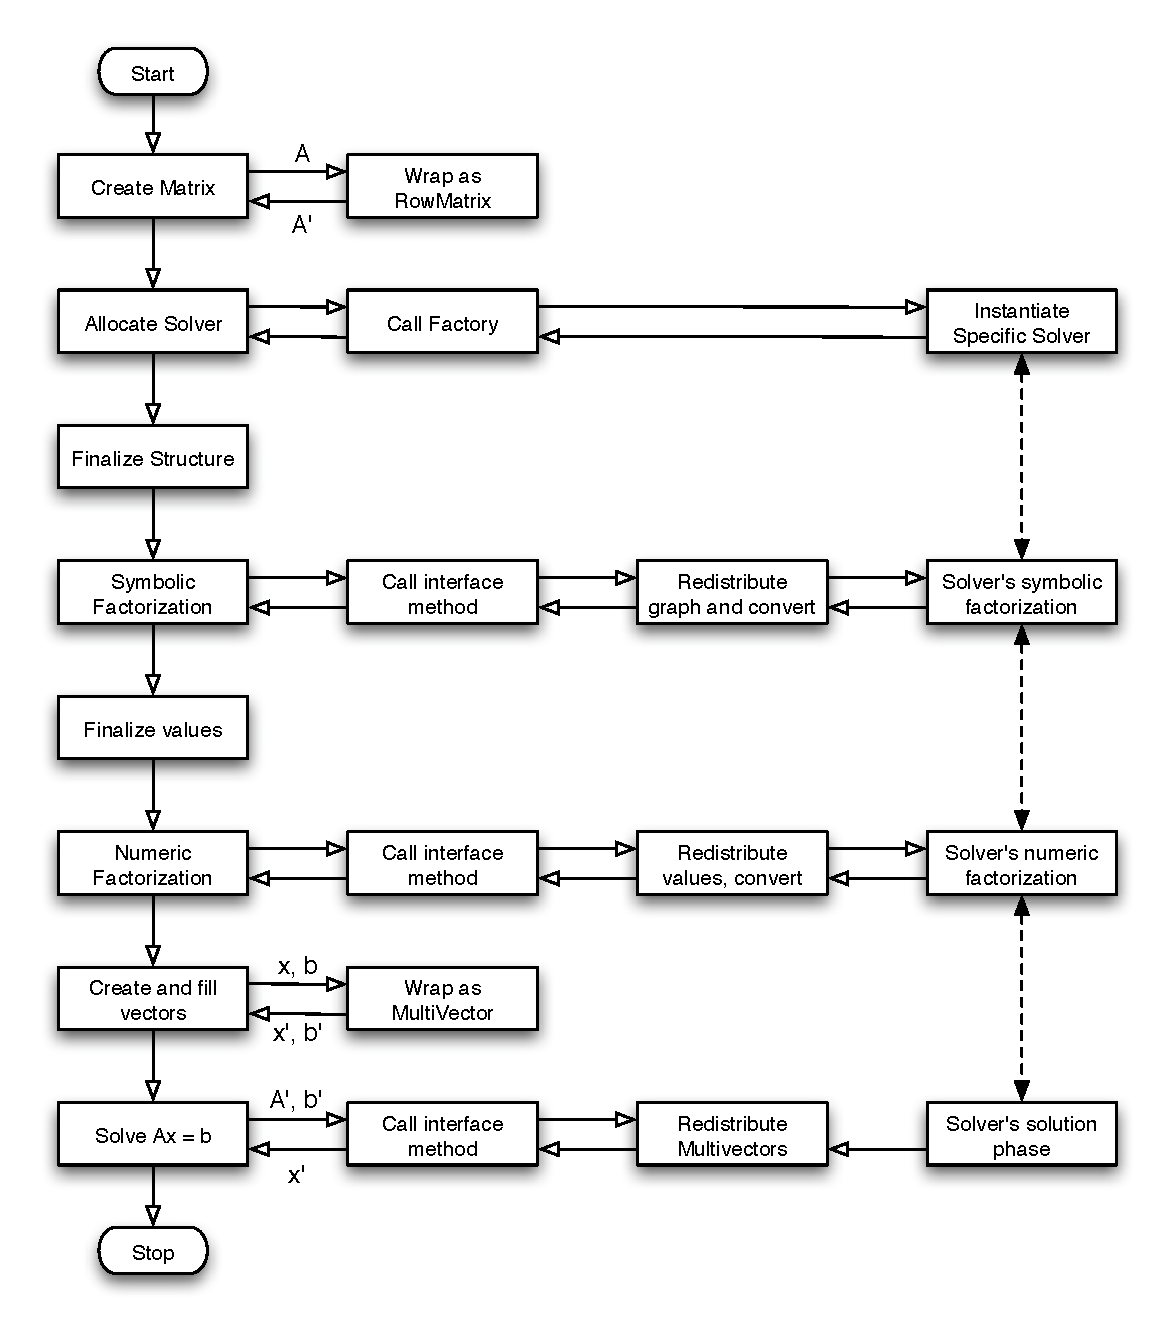
\includegraphics[width=12cm]{amesos_flowchart.eps}}
\end{center}
\caption{Flowchart.}
\label{fig:flowchart}
\end{figure}

\begin{figure}
\begin{center}
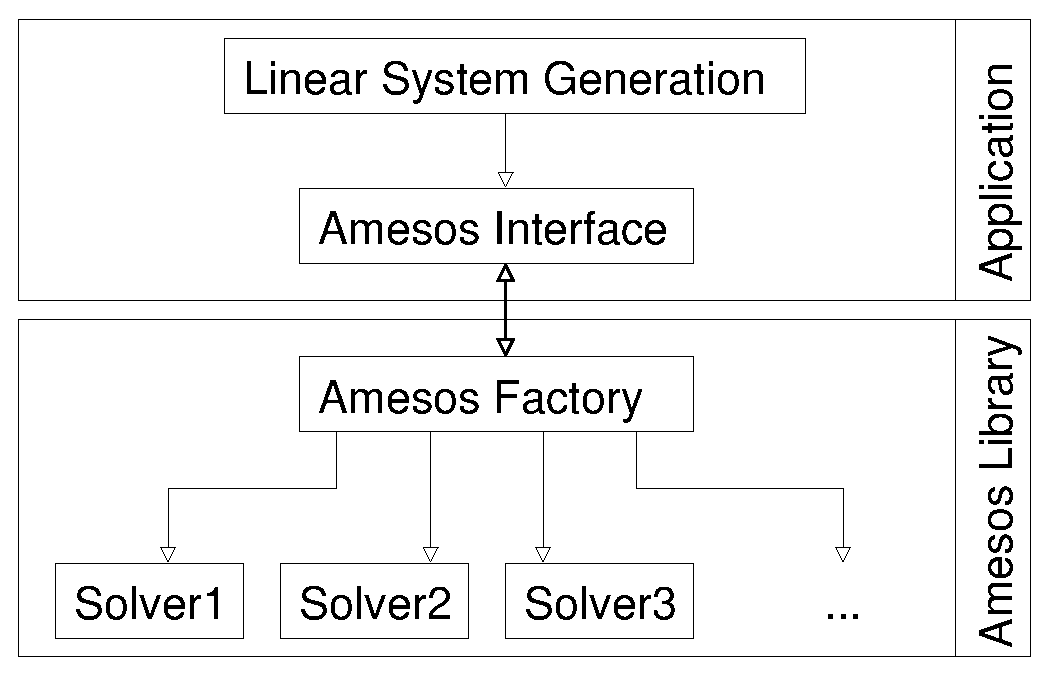
\includegraphics[width=7cm]{amesos_and_application.eps}
\end{center}
\caption{Connection between a generic application and Amesos.}
\label{fig:app}
\end{figure}

{\bf to be moved elsewhere...}

We want the application  code not only to manipulate BaseSolver objects 
(which can be done in an abstract way by using virtual member function and
 polymorphism), but also to create them without referring to the derived
classes. 
A very convenient and extensible way to create (abstract) solver objects is
through {\sl object factories}. Object factories are a programming
tool (see~\cite{alexandrescu04modern}) that implement a sort of ``virtual
constructor,'' in the sense that one can instantiate a generic derived object
while still working with abstract types.

The factory class simply looks like:
\begin{verbatim}
class Factory
{
  public:
    BaseSolver* Create(string type, <params>)
    {
      if (type == "solver1")
        return(new Solver1(<params>));
      else 
        ...
    }
};
\end{verbatim}
where \verb!<params>! is a generic list of parameters, and \verb!Solver1! is a
BaseObject derived class. 

Of course, one could in principle directly construct the required BaseSolver
objects in the application code; however, this would mean:
\begin{itemize}
\item it collects in one application source file knowledge about
Amesos-supported solvers;
\item most Amesos header files have to be included, and this automatically
includes the header files of the supported libraries;
\item it is hard to extend and maintain up-to-date.
\end{itemize}



%------------------------------------------------------------------------- 
\section{A Concrete Implementation}
\label{sec:concrete}
%------------------------------------------------------------------------- 

We now describe a concrete implementation of the proposed framework, as
available in the {\sl Amesos} package of the Trilinos
project~\cite{heroux05trilinos,trilinos-home-page}.
Amesos, developed by (in alphabetical order) T. Davis,
M. Heroux, R. Hoekstra, M. Sala, and K. Stanley, is an effort to define a set
of object-oriented, abstract interfaces for the usage of serial and
parallel sparse direct solvers. 
Amesos interfaces to the following third-party serial and parallel sparse
direct solvers: UMFPACK, PARDISO, TAUCS, SuperLU, SuperLU\_DIST, MUMPS,
DSCPACK. It also offers support for two dense solvers:
LAPACK~\cite{lapack-guide} and
ScaLAPACK~\cite{scalapack-guide}.
This section gives a brief overview of Amesos; for more details, we
refer to~\cite{Amesos-Reference-Guide}.



%-----------------------------------------------------------------------------
\subsection{An Example of Usage}
\label{sec:basic}
%-----------------------------------------------------------------------------

{\bf REPORT A COMPLETE EXAMPLE USING EPETRA....}

A fragment of code using Amesos is as follows.
Let us suppose that \verb!A! is an \verb!Epetra_RowMatrix!, and \verb!X! and
\verb!B! are two \verb!Epetra_MultiVector!'s. 
First,
  we need to include the header files for Amesos:
\begin{verbatim}
#include "Amesos.h"
#include "Amesos_BaseSolver.h"
\end{verbatim}
Note that these header files will {\sl not} include the header files for the
supported libraries (which are of course needed to compile the Amesos
library itself).  Then, we need to create an linear problem, as follows:
\begin{verbatim}
Epetra_LinearProblem Problem(&A, &X, &B);
\end{verbatim}
To make the usage of Amesos simpler, we have written a Factory
class~\cite{xxx}.
At this point, we can create an Amesos class using the factory class
\verb!Amesos!:
\begin{verbatim}
Amesos_BaseSolver* Solver;
Amesos Factory;
char* SolverType = "Amesos_Klu"; // uses the KLU direct solver
Solver = Factory.Create(SolverType, Problem);
\end{verbatim}
At this point, we can perform the symbolic factorization
of the linear system matrix:
\begin{verbatim}
Solver->SymbolicFactorization();
\end{verbatim}
This phase does not require the numerical values of \verb!A!, which can
therefore be changed after the call to \verb!SymbolicFactorization()!.
However,  the nonzero pattern of \verb!A! {\em cannot} be
changed.
The numeric factorization is performed by
\begin{verbatim}
Solver->NumericFactorization();
\end{verbatim}
\verb!NumericFactorization()! accesses the values of \verb!A!, but does not
consider the vectors \verb!X! and \verb!B!. Finally, to solve the linear
system, we simply write
\begin{verbatim}
Solver->Solve();
\end{verbatim}

In the previous example, we showed how to use the SuperLU solver; other
interfaces
can be created using the factory class by simply changing one parameter. Note
that the supported solver can be serial or parallel, dense or sparse: the user
code still remains the same (except for the name of the solver); Amesos will
take care of data redistribution if required by the selected solver. The list
of supported solvers is reported in Section~\ref{sec:review}.
 Method
\verb!Factory.Query()! can be used to query the factory about the
availability of a given solver:
\begin{verbatim}
char* SolverType = "Amesos_Superlu";
bool IsAvailable = Factory.Query(SolverType);
\end{verbatim}

\bigskip

Graph theory ideas can be used to pre-process a sparse matrix to arrage it in
desiderable patterns so that further computations are easy and fast; a that
the numerical algorithm goes better (e.g. ILU). Reordering is a very well-know
technique for direct solvers, see for example [Duff, erisman, reid, direct
methods for sparse matrices, clarendon press, 1986].

%-----------------------------------------------------------------------------
\subsection{Local Solvers in Domain Decomposition Preconditioners}
\label{sec:ifpack}
%-----------------------------------------------------------------------------

For an abstract point of view, an algebraic domain decomposition
preconditioner for the iterative solution of the linear system
(\ref{eq:linear_system})
if any preconditioner $B$ that can be written as
\begin{equation}
\label{eq:prec}
B^{-1} = \sum_{i=1}^M P'_i {A'_i}^{-1} R_i.
\end{equation}
Let $V = \mathbb{R}^n$, and
let $V_i \subset V, i = 1, \ldots, M$ be a decomposition of $V$, such that
$\cup_{i=1}^M V_i = V$, and $R_i: V \rightarrow V_i$ a restriction operator
from $V$ to the subspace $i$ (of size $n_i$),
and $P_i: V_i \rightarrow V, P'_i : V_i \rightarrow V$ two prolongator
operators. $A'_i$ is an approximation to $A_i = R_i A P_i$. 

Preconditioners of type (\ref{eq:prec}) constitute an example of one-level
domain decomposition preconditioners if the spaces $V_i$ are properly chosen,
so that each $V_i$ contains the unknowns defined on $\Omega_i$, a contiguous
subset of the computational domain $\Omega$. Parallelizing (\ref{eq:prec})
is simply obtained by assigning each subdomain to a different processor.
Often, parallel codes adopt a similar approach to distribute the linear
system matrix, making (\ref{eq:prec}) a natural candidate for the definition
of the preconditioner.

The first domain decomposition algorithm has been proposed in 1870 by Schwarz
to prove the solution of PDE problems on complex shape domains. In modern
terms, they have been re-discovered in the late 80's, and since then widely
used by pure mathematicians and computer scientists. We refer to
monographs~\cite{QV2,smith96parallel} for a detailed
overview of domain decomposition methods, to~\cite{saad96iterative} for the
algebraic interpretation,
  
\smallskip

Several recent projects have addressed the definition of parallel algebraic
domain decomposition preconditioners. Among the most successful, we here
recall the Aztec library~\cite{Aztec}, the PETSc library~\cite{petsc-guide}.
If a solver creates the local matrix $A_i'$ using a format that satisfies
Interface~\ref{int:ami}, then using Interface~\ref{int:asi} one can access a
variety of (local) direct solvers. This is done, for example, by the IFPACK library.

%-----------------------------------------------------------------------------
\subsection{Coarse Solver in Multilevel Methods}
\label{sec:ml}
%-----------------------------------------------------------------------------

The ML project aims to define multilevel preconditioners, in particular of
algebraic type; see for instance \cite{brandt.classic}, \cite{hack.book}, or
\cite{hack2.book}.
A multigrid solver tries to approximate
the original PDE problem of interest on a hierarchy of grids and use
`solutions' from coarse grids to accelerate the convergence
on the finest grid.  
Here, our interest is on the solution of the coarse
problem, which is usually performed with a direct solution method. If the
multigrid solver implements Interface~\ref{int:ami}, then it can use the {\tt
Solver} class to access {\sl any} supported direct solver, with no need to
code an adaptor to the direct library of choice. Because of the {\tt
Redistributor} class, one can tune the number of processors used in the
solution of the coarse problem, thus optimizing performances. An example of
multilevel solver that implements Interface~\ref{int:ami} is
ML~\cite{ml-guide} and it API, MLAPI~\cite{sala05object}.

%-----------------------------------------------------------------------------
\subsection{Testing with a Scripting Language: The Python Interface}
\label{sec:pytrilinos}
%-----------------------------------------------------------------------------

Another advantage of the presented set of interface is that is it (relatively)
  easy to use them from a scripting language like Python by adopting tools
  like SWIG~\cite{swig}. Since SWIG supports intra-language class inheritance,
  it is possible to derive Interface~\ref{int:ami} in Python, then pass it
  to the Python wrapper Inteface~\ref{int:asi}. This approach makes all the
  supported libraries available to Python developers at almost no cost. For
  more details, we refer to the PyTrilinos
  documents~\cite{sala05pytrilinos,pytrilinos-la-guide}. 
  
%-----------------------------------------------------------------------------
\section{Concluding Remarks}
\label{sec:conclusions}
%-----------------------------------------------------------------------------

In this paper, we have presented a model to access direct
solver libraries. The model is composed by two abstract interfaces, one to
access the matrix elements, and the other to manage each library.
The advantages of this model are:
\begin{itemize}

\item The actual data storage of linear system matrix becomes inessential.
Each concrete implementation will take care, if necessary, to convert the
input matrix into the required data format, should the row access provided by
\verb!GetMyRow()! method be not sufficient. This means that the
application can choose the matrix format independently as long as the abstract
matrix interface is implemented.

\item Issues like diagonal perturbations, reordering or dropping before the
 factorization can easily introduces within the AMI. For example, a dropping
 strategy simply requires a new \verb!GetMyRow()! method --- without
 touching the actual matrix storage.

\item The actual calling sequence required by each library to factorize the
matrix and solve the linear system becomes inessential. Instead, the user only
has to call methods \verb!Initialize()!, \verb!Compute()! and
\verb!Solve()!.

\item Adaptors can be tested more easily because they are all located within
the same library and not spread out into several application codes.
\end{itemize}

Clearly,  generalities comes at a price: the presented model has the following
limitations:
\begin{itemize}
\item 
Each adaptor automatically selects the default parameters defined by the
supported solver. In most cases, these values are a robust and reliable choice
for most applications. If required, the user can tune some of the parameters
by using method \verb!SetParameters()!. However, some fine-tuning can be
difficult since Interface~\ref{int:asi} has no knowledge of the underlying
solver data structure.

\item There
  is no standard way to 
  convert MPI communicators defined in C to MPI communicators defined
  in FORTRAN90. On some architectures it is difficult or even
  impossible to perform such a task. Some hacks may be required.

\item It can be difficult to support single precision and complex arithmetics.
At present, only double precision is supported by the Amesos project. 
Although the model can in
principle support single precision and complex arithmetics 
(by using templates, for example), no code
that implements Interface~\ref{int:asi} has been written yet. A templated
version of Interface~\ref{int:ami} is under development within the Tpetra
package.

\item 
It is almost impossible to support different versions of a given software
library, because
function names usually do not vary from one version to the
next, making it impossible for the linker to select the
  appropriate version of the library.

\item 
Not all adaptors can be compiled and linked at the same time. Often
developers of direct solver libraries take advantage of other, smaller
libraries, that offer common functionalities. Typically, this happens with
reordering algorithms. Unfortunately,
  it is not uncommon for different solver libraries to request different
  versions of a given reordering algorithm, all codes using the same function
  names. As a result, not all the adaptors can be compiled and used at the
  same time.
\end{itemize}

The reader might wonder why we have limited our attention to direct methods only, and
we did not include iterative methods as well in the definition of the abstract
interfaces. The reason is that, although
being often more performant in terms of CPU time and memory usage, iterative
solvers are less robust and mich less black-box than direct methods. Most
iterative methods are developed for PDE-like problems, and might have poor
performances if applied to more general matrices. However, libraries based on
the abstract matrix interface exist.

\bigskip

Talk about:

-SQA: debugged interfaces

-automated testing/ better documentation

- autoconf/autotools to make these interfaces portable...

\begin{table}
\begin{center}
\begin{tabular}{|l r r r| r r r|}
\hline
\multicolumn{4}{| c |}{Matrix} &
\multicolumn{3}{ c |}{Interface Time / Solver Time * 100} \\
Name  & $n$   & $nnz$  & $nnz / n$  & KLU     & UMFPACK   & SuperLU \\
\hline
\tt FIDAP001 & 216   &   4374 & 20.25 & 23.5   & 6.89  & 4.89  \\
\tt FIDAP002 & 414   & 26831  & 60.84 & 26.6   & 7.92  & 5.96  \\
\tt FIDAP003 & 1821  & 52659  & 28.91 & 18.5   & 4.94  & 2.64  \\
\tt FIDAP004 & 1601  & 32287  & 20.16 & 1.47   & 4.40  & 2.81  \\
\tt FIDAP005 & 27    & 279    & 10.33 & 112.52 & 28.5  & 8.46  \\
\tt FIDAP006 & 1651  & 49479  & 29.96 & 1.03   & 7.17  & 2.14  \\
\tt FIDAP007 & 1633  & 54487  & 33.36 & 12.8   & 2.07  & 1.59  \\
\tt FIDAP008 & 3096  & 106302 & 34.33 & 10.8   & 0.931 & 0.789 \\
\tt FIDAP009 & 3363  & 99397  & 29.55 & 14.6   & 4.78  & 0.863  \\  
\tt FIDAP010 & 2410  & 54816  & 22.74 & 25.78  & 6.43  & 4.75  \\  
\tt FIDAP011 & 16614 &1091362 & 65.68 & 0.120  & 0.701 & 0.111 \\  
\tt FIDAP012 & 3973  & 80151  & 20.17 & 0.216  & 3.34  & 2.07  \\  
\tt FIDAP013 & 2568  & 75628  & 29.45 & 18.31  & 12.1  & 2.59  \\  
\tt FIDAP014 & 3251  & 66647  & 20.50 & 0.172  & 1.71  & 1.94  \\  
\tt FIDAP015 & 6867  & 96421  & 14.04 & 10.480 & 4.38  & 2.89  \\  
\tt FIDAP018 & 5773  & 69335  & 12.01 & 8.18   & 2.73  & 2.14  \\  
\tt FIDAP019 & 12005 & 259863 & 21.64 & 15.17  & 4.23  & 3.34  \\  
\tt FIDAP020 & 2203  & 69579  & 31.58 & 1.32   & 5.89  & 1.77  \\  
\tt FIDAP021 & 656   & 19142  & 29.17 & 6.84   & 9.52  & 5.68  \\  
\tt FIDAP022 & 839   & 22613  & 26.95 & 6.50   & 6.76  & 8.92  \\
\tt FIDAP023 & 1409  & 43481  & 30.85 & 0.934  & 5.26  & 4.13  \\
\tt FIDAP024 & 2283  & 48733  & 21.34 & 2.11   & 4.09  & 3.55  \\
\tt FIDAP025 & 848   & 24532  & 28.92 & 9.93   & 4.29  & 4.04  \\
\tt FIDAP026 & 2163  & 93749  & 43.34 & 0.724  & 4.16  & 2.59  \\
\tt FIDAP027 & 974   & 40736  & 41.82 & 5.25   & 5.10  & 4.02  \\
\tt FIDAP028 & 2603  & 77653  & 29.83 & 0.896  & 4.08  & 3.81  \\
\tt FIDAP029 & 2870  & 23754  & 8.276 & 9.95   & 3.81  & 2.44  \\
\tt FIDAP031 & 3909  & 115299 & 29.49 & 0.575  & 3.75  & 3.51  \\
\tt FIDAP032 & 1159  & 11343  & 9.786 & 0.791  & 3.87  & 4.84  \\
\tt FIDAP033 & 1733  & 20315  & 11.72 & 15.89  & 4.58  & 13.1   \\
\tt FIDAP035 & 19716 & 218308 & 11.07 & 8.56   & 2.74  & 2.53  \\
\tt FIDAP036 & 3079  & 53851  & 17.48 & 2.03   & 4.30  & 3.35  \\
\tt FIDAP037 & 3565  & 67591  & 18.95 & 11.08  & 4.58  & 3.15  \\
\tt FIDAPM02 & 537   & 19241  & 35.83 & 14.74  & 3.67  & 2.42  \\
\tt FIDAPM03 & 2532  & 50380  & 19.89 & 1.00   & 4.33  & 1.61  \\
\tt FIDAPM05 & 42    & 520    & 12.38 & 82.85  & 16.3  & 8.40  \\
\tt FIDAPM07 & 2065  & 53533  & 25.92 & 0.602  & 1.52  & 1.15  \\
\tt FIDAPM08 & 3876  & 103076 & 26.59 & 0.220  & 3.36  & 1.08  \\
\tt FIDAPM09 & 4683  & 95053  & 20.29 & 0.536  & 2.45  & 2.21  \\
\tt FIDAPM10 & 3046  & 53842  & 17.67 & 9.979  & 3.82  & 3.72  \\
\tt FIDAPM11 & 22294 & 623554 & 27.96 & N/C    & 0.17  & 0.403 \\
\tt FIDAPM03 & 3549  & 71975  & 20.28 & 0.355  & 3.59  & 0.919 \\
\tt FIDAPM05 & 9287  & 98519  & 10.60 & 42.90  & 2.59  & 2.03  \\
\tt FIDAPM29 & 13668 & 186294 & 13.62 & 0.869  & 2.511 & 1.57  \\
\tt FIDAPM33 & 2353  & 23765  & 10.09 & 0.6560 & 3.39  & 3.47  \\
\tt FIDAPM37 & 9152  & 765944 & 83.69 & 2.247  & 2.87  & 0.585 \\
\hline
\end{tabular}
\caption{Additional time required by the Amesos interface with respect to the
time required by the solver, for different matrices and solvers. $n$
  represents the size of the matrix, and $nnz$ the total number of nonzeros.
The results were obtained on a G4 1.67 GHz with 1 GByte of RAM.}
\label{tab:interface}
\end{center}
\end{table}

{\bf to be moved somewhere else...}

We have preseted a set of reusable components... These generic components bring their
users the well-known benefits of libraries. Because of their high-level,
      generic components make it possible to connect intricate and complex
      application codes to complex linear solver libraries, in a simple and
      easy-to-maintain way. The elements we have used are: object-oriented
      design, a little bit of  generic programming, and C++. These elements
      are combined to achieve a high rate of reuse, for both the point of view
      of the application and of the supported libraries. For the application,
      the small amount of required code makes it very convenient to use
      Amesos. The generality of the components make them applicable to a vast
      range of applications.
      

%-----------------------------------------------------------------------------%
\bibliographystyle{acmtrans}
\bibliography{paper}
%-----------------------------------------------------------------------------%

\end{document}
